\subsection{Feature selection}
To evaluate the impact of exogenous variables, several feature groups were individually tested and compared against a baseline model without features. The results are shown in Table~\ref{tab:sarimax_features}.

\begin{table}[h]
\centering
\begin{tabular}{l c c c c}
\hline
Feature Group & MSE (non-seasonal) & MSE (Seasonal) \\
\hline
no features (ARIMA) & 0 14.1044827 & 9.468997 \\
roll\_mean\_14 3.297528 & 2.856444 \\
roll\_mean\_7 & 3.376438 & 2.806345 \\
lag1            & 4.419191 & 3.171155 \\
dayofweek      & 4.653446 & 3.861770 \\
lag7           & 5.159591 & 3.875142 \\
roll\_std\_7    & 5.431850 & 3.761796 \\
month          & 5.503093 & 4.026655 \\
is\_weekend    & 7.708808 & 4.674045 \\
holiday        & 8.571233 & 4.860423 \\
\hline
\end{tabular}
\caption{Feature group performance comparison (lower MSE is better)}
\label{tab:sarimax_features}
\end{table}


The results show that exogenous features significantly improve forecasting performance compared to the baseline model without features. Rolling mean features achieved the lowest MSE values for both the seasonal and non-seasonal datasets, indicating that recent historical averages contain strong predictive information. 

The large reduction in MSE when using exogenous variables suggests that the forecasting problem is primarily driven by external or engineered features rather than strong autoregressive structure.

 \begin{figure}[h]
    \centering
    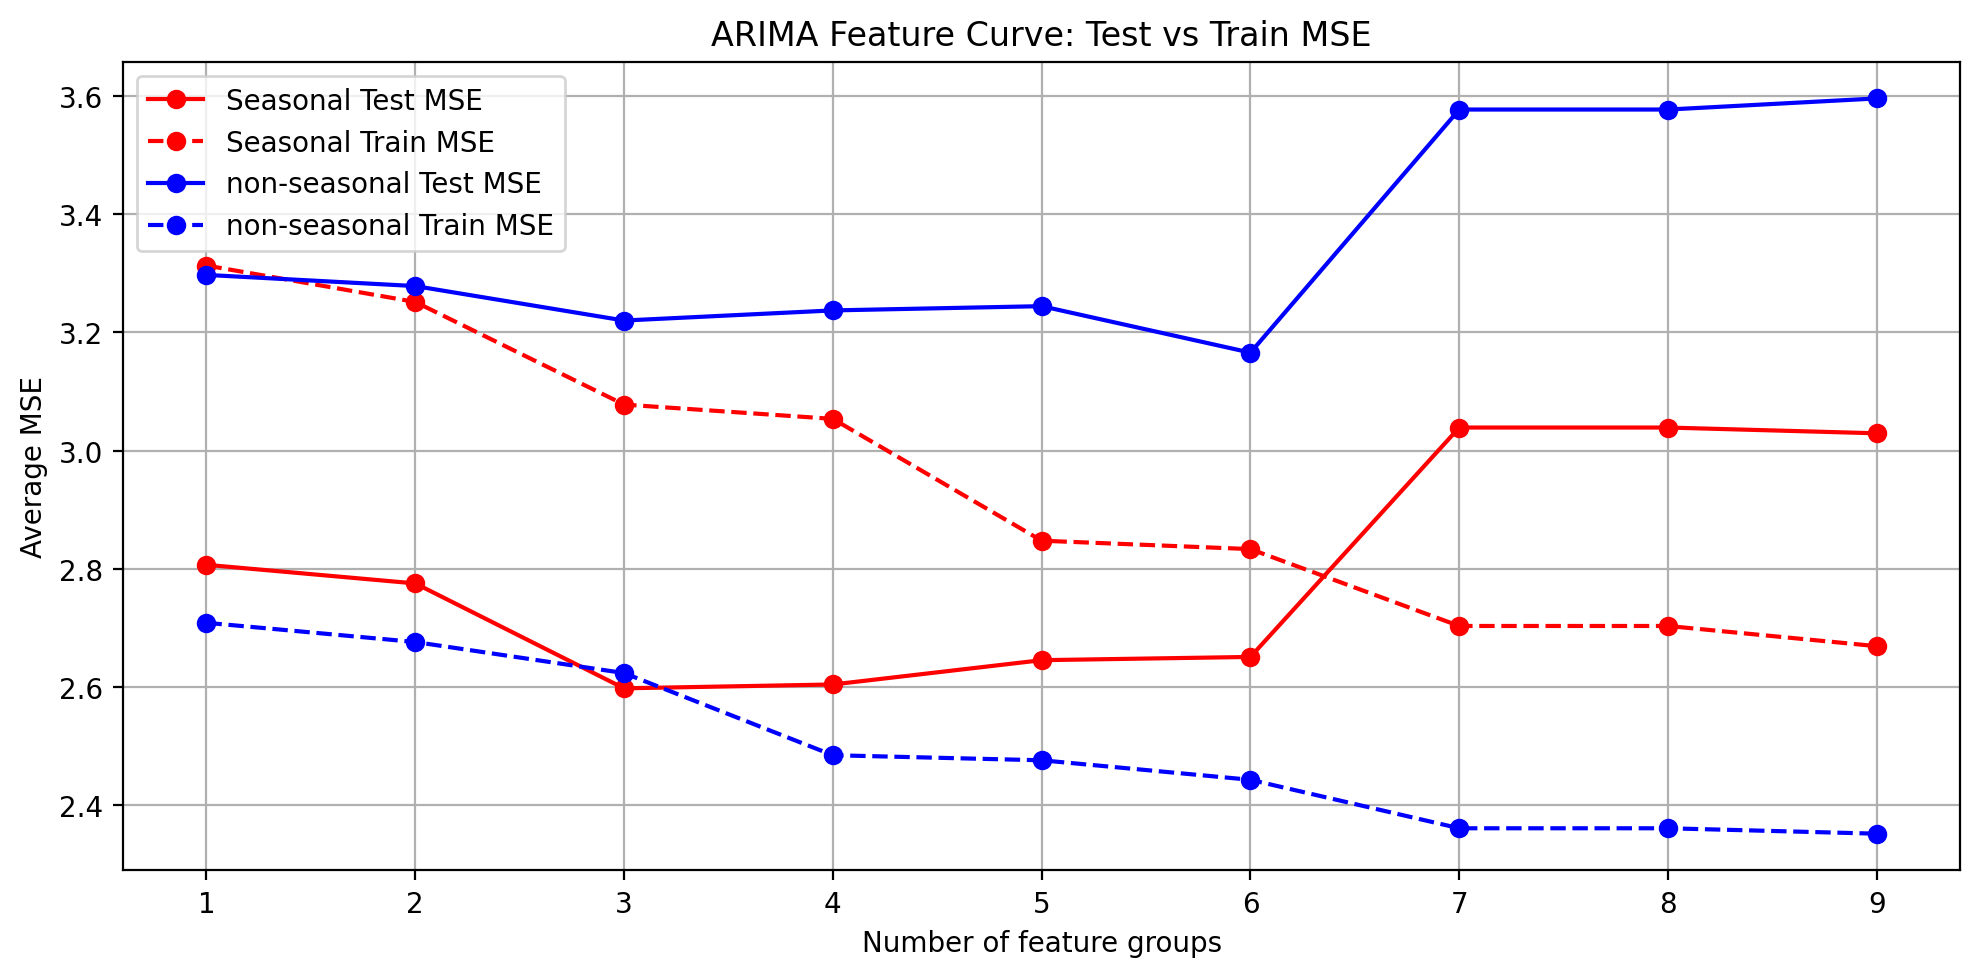
\includegraphics[width=\linewidth]{figures/feature_curve_combined.png}
    \caption{Feature Curve}
    \label{fig:mse_per_feature_added}
\end{figure}

Figure~\ref{fig:mse_per_feature_added} shows the training and test MSE as features are added incrementally. The features were added in the order of their individual performance shown in Table~\ref{tab:sarimax_features}.

For both datasets, the training MSE decreases consistently as more features are added. However, the test MSE only improves up to a certain point before beginning to increase. This behavior indicates overfitting, where the model starts fitting noise in the training data rather than learning patterns that generalize well to unseen data.

The lowest test MSE for the non-seasonal dataset was achieved using six features, while the seasonal dataset achieved its best performance using three features. 

Auto ARIMA was applied again after including the selected exogenous features for each dataset. In both the seasonal and non-seasonal cases, the optimal ARIMA configuration was found to be $(0,0,0)(0,0,0)$.

This indicates that, once the exogenous features are included, the model no longer benefits from autoregressive, differencing, moving average, or seasonal terms. In other words, the dependencies in the series are largely explained by the external features rather than by the historical structure of the time series itself.

These results suggest that the forecasting problem is primarily feature-driven, and that a simpler regression-based approach, such as Ordinary Least Squares (OLS), may be more appropriate than a full ARIMA-based model. Which we will look at in the next section. 

\begin{figure}[h]
    \centering

    \begin{subfigure}{\linewidth}
        \centering
        \includegraphics[width=\linewidth]{figures/arima_pred_seasonal.png}
        \caption{ARIMA forecasting seasonal cell}
        \label{fig:arima_forecasting_r_cell}
    \end{subfigure}


    \begin{subfigure}{\linewidth}
        \centering
        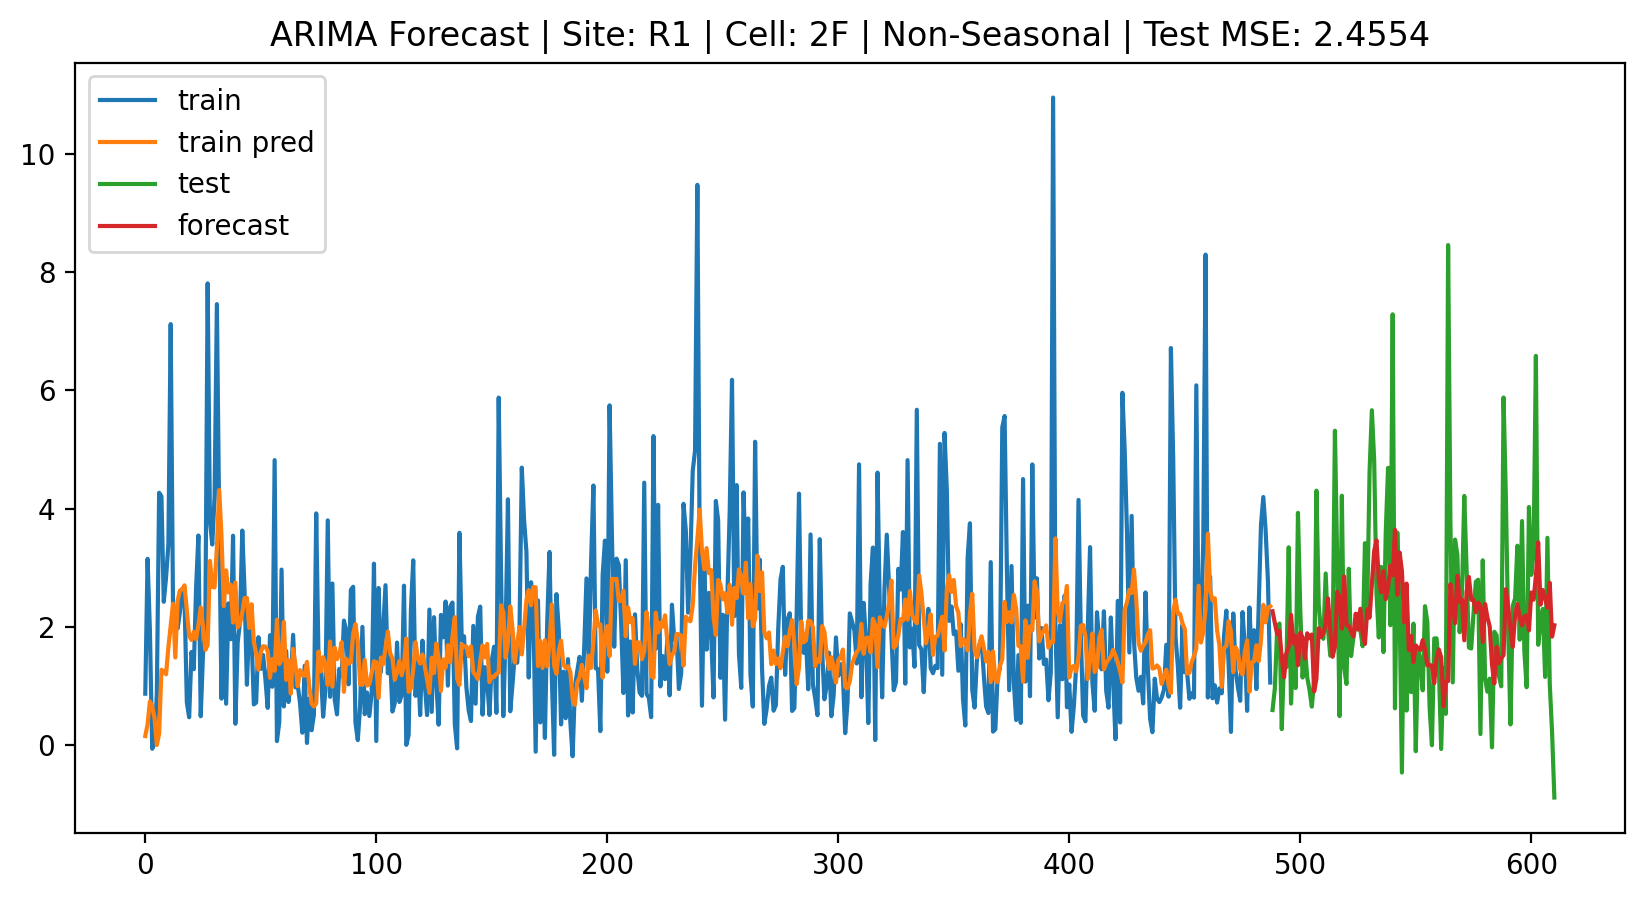
\includegraphics[width=\linewidth]{figures/arima_pred_non-seasonal.png}
        \caption{ARIMA forecasting non-seasonal cell}
        \label{fig:arima_forecasting_u_cell}
    \end{subfigure}

    \caption{Average data volume across cells for two towers}
    \label{fig:tower_data_avg}
\end{figure}